\documentclass{article}
\usepackage[utf8]{inputenc}
\usepackage{polski}
\usepackage{titlesec}
\usepackage[labelsep=period]{caption}
\usepackage{graphicx}
\usepackage{float}

\titlelabel{\thetitle.\quad}
\graphicspath{{/}}

\title{Sprawozdanie z dodatkowego zadania\\ - implementacja uniwersalnego algorytmu planowania procesów}
\author{Sławomir Górawski}
\date{23 stycznia 2018}

\begin{document}

\maketitle

\section{Wstęp}

Planowanie przydziału procesora polega na określeniu kolejności, w jakiej jego moc obliczeniowa zostanie przydzielona procesom z kolejki procesów gotowych do działania. Jest to zadanie planisty krótkoterminowego, który powinien zmaksymalizować czas wykorzystania procesora. Za każdym razem, gdy aktywny proces przechodzi w stan oczekiwania lub kończy działanie, podejmuje decyzję, którym procesem z kolejki gotowych do działania (jeśli ta jest niepusta) go zastąpić. Wynik tej decyzji zależy od działania zaimplementowanego algorytmu przydziału procesora.
\\\\
Algorytmy te można podzielić na:

\begin{enumerate}
    \item Niewywłaszczeniowe
    
    Decyzje planisty podejmowane są, gdy:
    \begin{itemize}
        \item aktywny proces przechodzi w stan oczekiwania,
        \item aktywny proces kończy działanie.
    \end{itemize}
    
    \item Wywłaszczeniowe
    
    Decyzje planisty podejmowane mogą być również, gdy:
    \begin{itemize}
        \item proces przechodzi ze stanu oczekiwania w stan gotowości,
        \item aktywny proces przechodzi w stan gotowości.
    \end{itemize}
\end{enumerate}

Strategie planowania można oceniać z różnych punktów widzenia. Głównym, choć nie jedynym, kryterium branym pod uwagę w tym sprawozdaniu będzie średni czas oczekiwania procesów gotowych do działania. Poniżej skrótowo omówione zostały algorytmy przetestowane w symulatorze. 

\section{Krótki opis algorytmów}

\subsection{FCFS}

FCFS (ang. \textit{first-come, first-served}) oznacza ``pierwszy zgłoszony - pierwszy obsłużony''. Algorytm ten opiera się na prostej zasadzie, zgodnie z którą procesy wykonywane są w takiej kolejności, w jakiej pojawiły się w kolejce gotowych do działania. Jest to algorytm niewywłaszczeniowy. Charakteryzuje się prostotą implementacji. Jego główną wadą jest stosunkowo długi średni czas oczekiwania, który jest skutkiem m.in. zjawiska znanego jako efekt konwoju (ang. \textit{convoy effect}), polegającego na blokowaniu procesów wymagających niewiele czasu do działania jednym długim.

\subsection{SJF}

SJF (ang. \textit{shortest job first}) preferuje procesy, które mają najmniejsze wymagania odnośnie czasu procesora. Jest to algorytm optymalny, jeśli chodzi o minimalizację średniego czasu oczekiwania. Może on być wywłaszczeniowy lub nie. W wersji wywłaszczeniowej, zwanej SRTF (ang. \textit{shortest remaining time first}), może zastąpić aktualnie wykonywany proces nowym, który pojawił się w kolejce, jeśli tylko tamten wymaga mniej czasu. Do jego wad należy możliwość zagłodzenia długich procesów, które mogą być wciąż pomijane na rzecz szybszych.

\subsection{RR}

RR (ang. \textit{Round-Robin}), czyli planowanie rotacyjne, to strategia, w której każdy proces otrzymuje kwant czasu procesora do wykorzystania. Po upływie tego czasu działanie procesu jest przerywane, a on sam jest przenoszony na koniec kolejki. Algorytm ten jest rzecz jasna wywłaszczeniowy i w porównaniu do innych powoduje znacznie więcej przełączeń kontekstu, poza tym dla procesów, które często zostają przerywane, łączny czas oczekiwania może być bardzo długi. Jego zaletą jest równomierne rozłożenie czasu działania pomiędzy wszystkie programy.

\section{Implementacja symulatora}

W pliku \texttt{program.ipynb} zaimplementowany został symulator planowania procesów, napisany w języku Python. Zasymulowane zostało w nim działanie omówionych powyżej algorytmów, tj. FCFS, SJF, SRTF i RR. Symulacja jest rzecz jasna uproszczona, nie zostały uwzględnione w niej np. czasy przełączania procesów, tym niemniej obserwacja jej działania pozwoliła wyciągnąć wiele wniosków dotyczących działania testowanych algorytmów.

Procesy zostały zaimplementowane jako klasy posiadające pola takie jak wymagany czas działania oraz łączny czas oczekiwania. Co pewną abstrakcyjną jednostkę czasu, odpowiadającą 1 ms czasu rzeczywistego, aktualizowana jest sytuacja w symulatorze. Działające procesy zmniejszą swój wymagany czas działania, zaś w chwili zakończenia pracy są zastępowane nowymi zgodnie z jedną z opisywanych wyżej strategii. Implementacje planistów opierają się głównie o metody decydujące, jak zastępować zakończone procesy.

Uniwersalność implementacji polega na jej modułowej budowie, łatwiej do rozszerzenia o kolejne algorytmy, oraz parametryzacji testów. Możliwość ustalenia przedziałów czasu wymaganego przez procesy, rozkładu prawdopodobieństwa czasu w przypadku jego losowania, kwantu czasu używanego przez algorytm RR itd. pozwoliła na sprawdzenie działania testowanych strategii w różnych sytuacjach, co nierzadko wpływało na zaobserwowane wyniki. 

\section{Wyniki}

Wyniki działania symulacji przedstawione zostały w postaci wypisywania średnich czasów oczekiwania procesów w przypadku konkretnych algorytmów, oraz prezentacji na wykresach przebiegu ich działania, gdzie poszczególnym punktom na wykresach odpowiadają procesy otrzymujące w danej chwili czas procesora, zaś ich wysokość odpowiada czasowi oczekiwania danego procesu w kolejce.
\\\\
Przykładowy wynik testu dla danych parametrów:
\\
\begin{table}[h]
    \centering
    \begin{tabular}{|l|r|}
        \hline
        łączny czas prowadzenia pomiarów & 1000 ms \\
        czas działania procesów & 20 - 40 ms \\
        rozkład prawdopodobieństwa & jednolity \\
        okres pojawiania się nowych procesów & 20 ms \\
        kwant czasu w algorytmie RR & 100 ms \\
        \hline
    \end{tabular}
    \caption{Parametry testu}
    \label{tab:test1param}
\end{table}

\begin{table}[h]
    \centering
    \begin{tabular}{|l|r|}
        \hline
        FCFS & 172,666667 \\
        SJF  & 38,216216 \\
        SRTF & 30,342857 \\
        RR   & 152,279279 \\
        \hline
    \end{tabular}
    \caption{Średni czas oczekiwania procesów [ms]}
    \label{tab:test1czas}
\end{table}

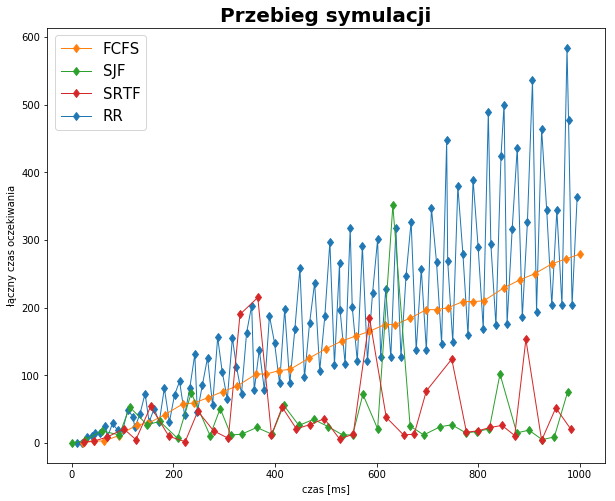
\includegraphics[scale=0.5]{plot}

\section{Wnioski}

Z powyżej przedstawionych wyników jednego z testów, a także kilku innych niezawartych w sprawozdaniu, można wyciągnąć kilka wniosków dotyczących planowania procesów. Niektóre z nich to:

\begin{itemize}
    \item algorytm SJF istotnie jest najlepszy, jeśli chodzi o średni czas oczekiwania,
    \item zaobserwować można występowanie problemu głodzenia dłuższych procesów w algorytmie SJF,
    \item zaobserwować można efekt konwoju w algorytmie FCFS,
    \item czas oczekiwania w algorytmie FCFS rośnie liniowo wraz ze wzrostem liczby procesów w kolejce,
    \item algorytm RR często zachowuje się podobnie jak FCFS, jednak wywłaszczanie procesów często znacznie wydłuża ich czas oczekiwania; tym niemniej średnio jest on i tak lepszy niż w przypadku algorytmu FCFS.
\end{itemize}

\end{document}
